\section{Dynamo}
\begin{frame}
  \frametitle{Dynamo: Amazon's Highly Available Key-value Store}
  Articolo di riferimento: \\
  \begin{thebibliography}{9}
  \bibitem{goldbach:congettura} DeCandia, G., Hastorum, D., Jampani, M., Kakalapati, G., Lakshman A., Pilchin, A.,
    Sivasubramanian, S., Vosshall, P. \& Vogels, W.
  \newblock Dynamo: Amazon's Highly Available Key-value Store
  \newblock \emph{ACM SIGOPS Operating Systems Review (Vol. 41, No. 6, pp. 205-220)}, (2007, October)
  \end{thebibliography}
\end{frame}

%DeCandia, G., Hastorun, D., Jampani, M., Kakulapati, G., Lakshman, A., Pilchin, A., ... & Vogels, W. (2007, October). Dynamo: amazon's highly available key-value store. In ACM SIGOPS Operating Systems Review (Vol. 41, No. 6, pp. 205-220). ACM.
\begin{frame}
  \frametitle{Dynamo}
  \begin{block}{Cos'è Dynamo}
  Dynamo è un sistema di key-value storage distribuito.
  \end{block}
  \begin{block}{Obiettivi}      
      \begin{itemize}
      \item ``Always on'' experience.
      \item Scalabilità.
      \item Alte performance - bassa latenza.
      \item Eventual consistency.
      \end{itemize}
  \end{block}
  In realtà il sistema è altamente configurabile, è possibile migliorare alcuni aspetti a scapito di altri...
\end{frame}


\begin{frame}
  \frametitle{Architettura del Sistema}
  Scomponiamo il sistema in base alle tecniche utilizzate:
  \begin{table}[ht]
  \begin{center} 
  \begin{tabular}{| l | l |}
  \hline
  \rowcolor{lightgray} 
  \textbf{Partizionamento e replicazione} & Consistent hashing \\
  \hline
  \textbf{Versionamento}                  & Vector clock \\
  \hline
  \rowcolor{lightgray}
  \textbf{Coerenza operazioni}            & Quorum likeness \\
  \hline
  \multirow{3}{*}{\textbf{Gestione fallimenti}}
                                          & Sloppy quorum, \\
                                          & hinted handoff, \\
                                          & Merkle tree \\ 
  \hline
  \rowcolor{lightgray}
  \textbf{Membership e rilevamento fallimenti}  & Gossip-based protocol, \\ 
  \hline
  \end{tabular}
  \end{center}
  \end{table}
\end{frame}


\begin{frame}
  \frametitle{Partizionamento (I)}
  \begin{itemize}
  \item Si usa la tecnica del \alert{consistent hashing}.
  \end{itemize}
  \begin{block}{Consistent hashing}
    \begin{itemize}
    \item Tabella hash richiusa ad anello.
    \item Nodi posizionati casualmente sull'anello a formare intervalli.
    \item Ogni nodo memorizza le chiavi nell'intervallo tra lui e il precedente.
    \end{itemize}
  \end{block}
  \begin{figure}
  \centering
  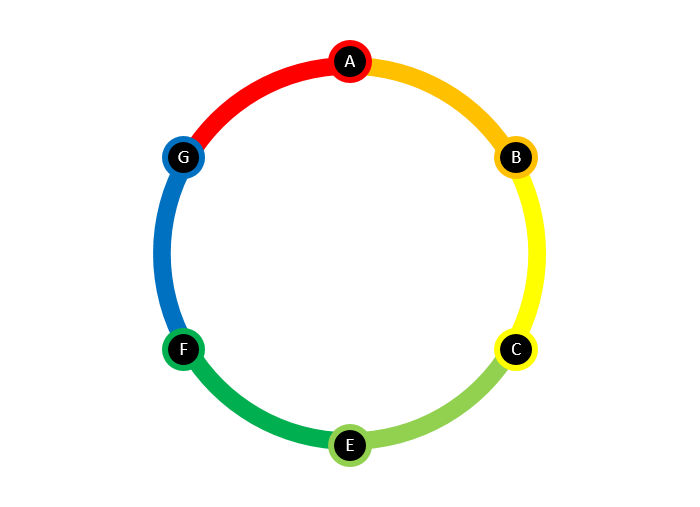
\includegraphics[scale=0.25]{dynamo/consistent-hashing-ring.png}
  \end{figure}
\end{frame}


\begin{frame}
  \frametitle{Partizionamento (II)}
  \begin{columns}
  \begin{column}{0.5\textwidth}
  Dynamo propone una variante del consistent hashing, utilizzo di \alert{nodi virtuali} (tokens).
  \end{column}
  \begin{column}{0.5\textwidth}
  \begin{figure}
  \centering
  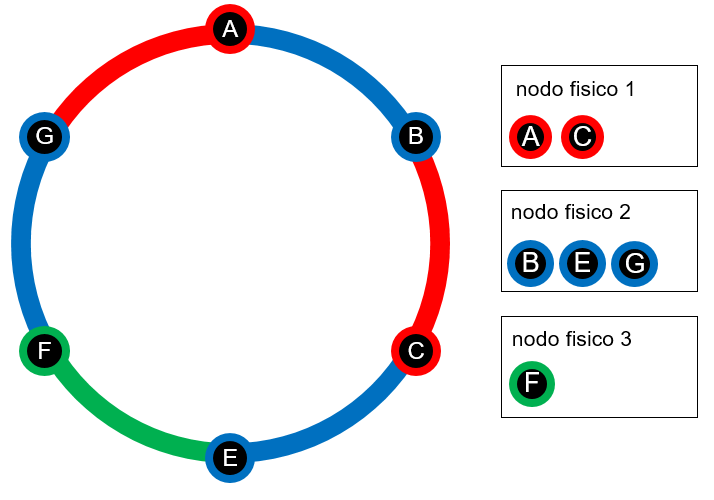
\includegraphics[scale=0.23]{dynamo/virtual-node.png}
  \end{figure}
  \end{column}
  \end{columns}
  \begin{block}{Vantaggi}
  \begin{itemize}
  \item Dati distribuiti uniformemente.
  \item Aggiungere o togliere nodi influenza solo il ``successore''.
  \item Bilanciamento del carico a seguito di un fallimento.
  \item Si tiene conto dell'eterogeneità delle macchine.
  \end{itemize}
  $\longrightarrow$ In poche parole si ottiene una forte \alert{scalabilità}.
  \end{block}
\end{frame}


\begin{frame}
  \frametitle{Replicazione}
  Ogni nodo effettua una replica sugli $N$ nodi successivi (senso orario).
  \begin{itemize}
  \item L'insieme dei nodi che ospitano il medesimo intervallo di chiavi è detto \alert{preference list}.
  \item I nodi virtuali sono saltati lungo l'anello.
  \item L'aggiornamente delle repliche è \alert{asincrono}.
  \end{itemize}
  \begin{figure}
  \centering
  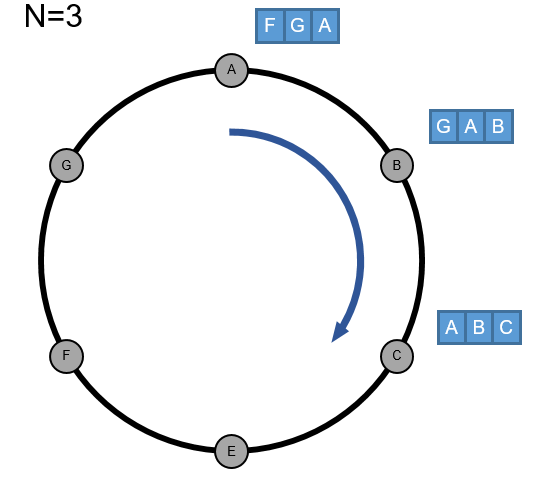
\includegraphics[scale=0.35]{dynamo/replication.png}
  \end{figure}  
\end{frame}


\begin{frame}
  \frametitle{Versionamento (I)}
  \begin{itemize}
  \item Ogni modifica viene trattata dal sistema come un nuovo oggetto.
  \item Si utilizzano i \alert{vector clock} ($\vclock$) per tenere traccia delle versioni:
  \end{itemize}
  \centering
    \[
    \big[<\mathrm{nodo}, \mathrm{counter}> <n_2, c_2> ... <n_m, c_m> \big]
    \]
    
  \begin{definizione}
    Siano $x$ e $y$ due versioni del medesimo oggetto, denotiamo con $\vclock(x)_z$ il vector clock di $x$ relativo al nodo $z$.
    \begin{multline*}
    \vclock(x) < \vclock(y) \iff \\
      \big( \forall z \mathrel{:} \vclock(x)_z \leq \vclock(y)_z \big) \land \big( \exists z' \mathrel{:} \vclock(x)_{z'} < \vclock(y)_{z'} \big) 
    \end{multline*}
  \end{definizione}
\end{frame}


\begin{frame}{Versionamento (II)}
  Si ottiene un ordinamento parziale sulle versioni:
  \begin{itemize}
  \item Se $\vclock(x) < \vclock(y)$ allora la versione $y$ può sovrascrivere $x$.
  \item Altrimenti abbiamo un branching delle versioni che il sistema non può riconciliare autonomamente.
  \end{itemize}
  
  Un esempio:
  \begin{figure}
  \centering
  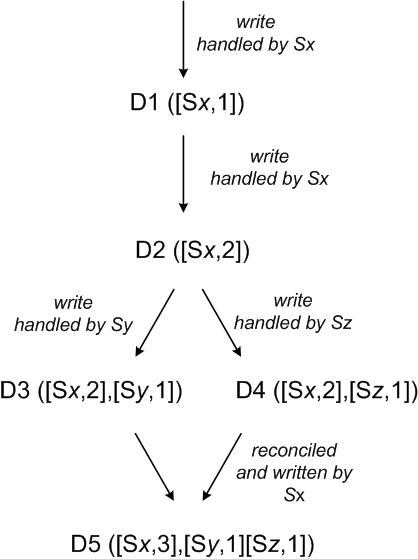
\includegraphics[scale=0.3]{dynamo/versioning.png}
  \end{figure}  
\end{frame}


\begin{frame}{Versionamento (III)}
  \begin{block}{Pro dell'uso dei vector clock}
    \begin{itemize}
    \item Rispetto all'utilizzo di un timestamp logico si ottiene un ordinamento parziale tra le versioni.
    \item I vari branch di versionamento vengono tutti individuati e ritornati per una riconcialiazione da parte del client.
    \end{itemize}
  \end{block}

  \begin{block}{Contro}
    \begin{itemize}
    \item La dimensione dei vector clock può crescere tanto...
    \item ...in realtà solo in casi di ripetuti fallimenti o partizionamento della rete.
    \end{itemize}
  \end{block}
\end{frame}


\begin{frame}
  \frametitle{Garantire la Coerenza}
  \begin{itemize}
  \item Operazione di \texttt{get} e \texttt{put}:
    \begin{itemize}
    \item \texttt{get(key) : <value, context>}
    \item \texttt{put(key, value, context)}
    \end{itemize}
  \end{itemize}
  \begin{itemize}
  \item La coerenza è ottenuta mediante la tecnica del \alert{quorum}:
    \begin{itemize}
    \item $W$: ($W \leq N$) numero di nodi che contribuiscono alla scrittura.
    \item $R$: ($R \leq N$) numero di nodi che contribuiscono alla lettura.
    \end{itemize}
  \end{itemize}
\end{frame}


\begin{frame}
  \frametitle{Operazione \texttt{get}}
  $N = 4, W = 2, R = 3$
  \begin{figure}
  \centering
  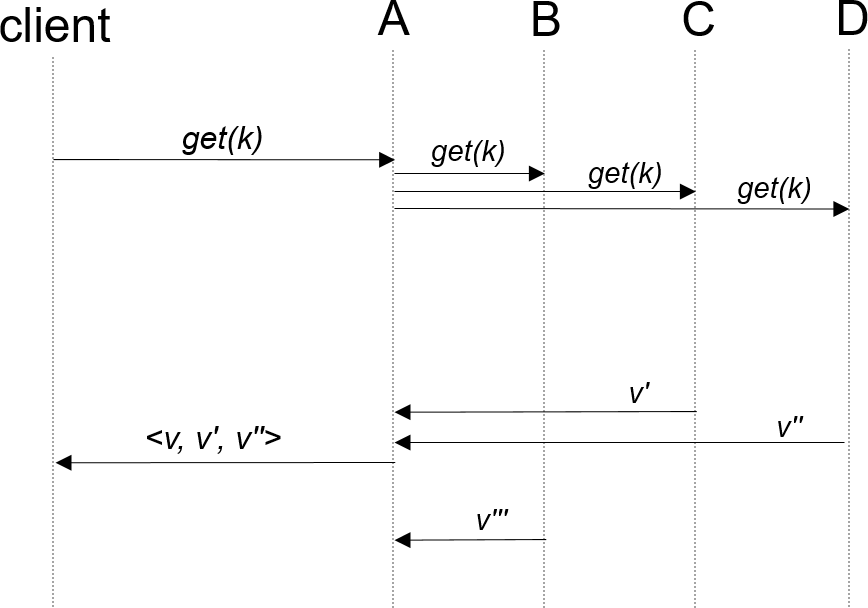
\includegraphics[scale=0.4]{dynamo/get.png}
  \end{figure}
\end{frame}


\begin{frame}
  \frametitle{Operazione \texttt{put}}
  $N = 4, W = 2, R = 3$
  \begin{figure}
  \centering
  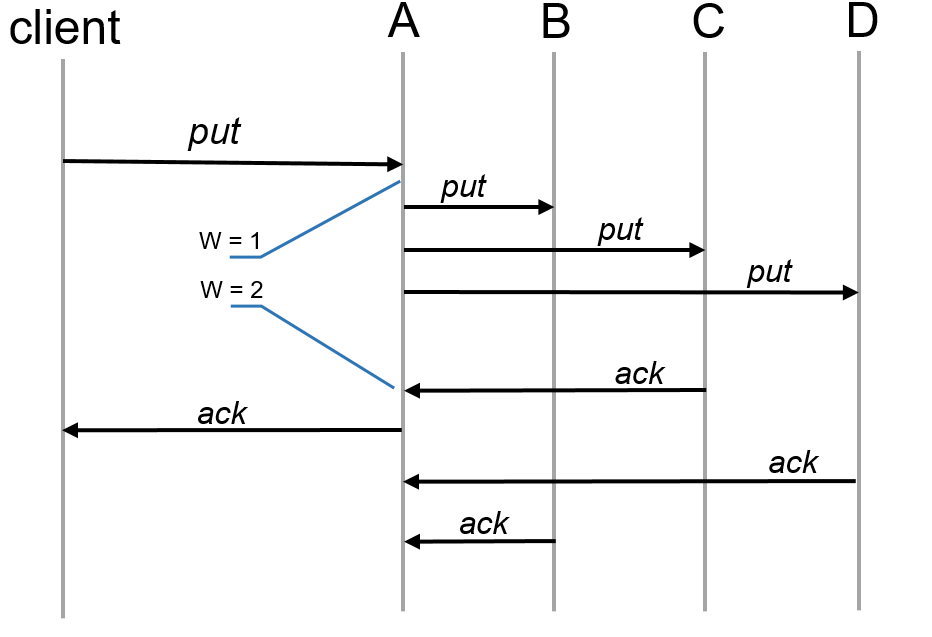
\includegraphics[scale=0.4]{dynamo/put.png}
  \end{figure}
\end{frame}


\begin{frame}
  \frametitle{Proprietà di un quorum-like system}
  \begin{block}{Se $R + W > N$}
    \begin{itemize}
      \item in assenza di fallimenti abbiamo \alert{strong consistency}.
    \end{itemize}
  \end{block}
  \begin{block}{Se $R + W \leq N$}
    \begin{itemize}
    \item ottengo \alert{eventual consistency} a vari livelli...
    \item $W = 1$: always writable (high availability).
    \item $R = 1$: always readable (high availability).
    \end{itemize}
  \end{block}
\end{frame}


\begin{frame}
  \frametitle{Rissumendo su $W, R$ e $N$}
  \begin{figure}
  \flushleft
  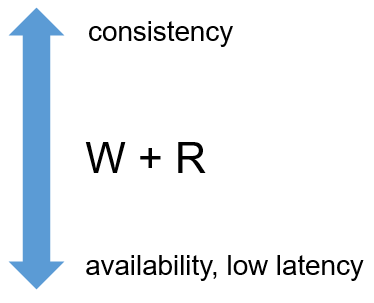
\includegraphics[scale=0.4]{dynamo/consistency-trade-off.png}
  \end{figure}
  \begin{block}{Esempio}
  \emph{High performance read engine}: Dynamo è pensato per essere un ``always writable'' data store, con $R=1$ e $W=N$ diventa un sistema ideale per servire tante letture con poche e rare scritture. 
  \end{block}
\end{frame}


\begin{frame}
  \frametitle{Sloppy Quorum}
  \begin{block}{Problema}
    Bastano pochi fallimenti nella ``top $N$'' della preference list per impedire il raggiungimento del quorum.    
  \end{block}
  \begin{block}{Si utilizza lo ``sloppy quorum'':}
  \begin{itemize}
  \item Durante un'operazione si contattano i primi $N$ nodi \alert{sani} nella preference list (si scorre in senso orario l'anello).
  \item La replica che normalmente risiederebbe sul nodo fallito viene traferita al nodo supplente.
  \end{itemize}
  \end{block}
  $\longrightarrow$ Quando i nodi falliti ritornano in servizio nasce un problema di incoerenza. 
\end{frame}


\begin{frame}
  \frametitle{Gestione Fallimenti e Sincronia Repliche (I)}
  \begin{block}{Hinted handoff}
  \begin{itemize}
  \item La replica spedita al nodo ``supplente'' contiene un \alert{hint}.
  \item Il nodo supplente si preoccupa di verificare periodicamente lo stato del nodo che sta sostituendo.
  \item Non appena possibile viene restituita la replica aggiornata al nodo fallito.
  \end{itemize}
  In questo modo si minimizza la finestra di vulnerabilità.
  \end{block}
\end{frame}

\begin{frame}
  \frametitle{Gestione Fallimenti e Sincronia Repliche (II)}
    In caso di fallimento di un supplente è necessario un mezzo per stabilire se due repliche sono sincronizzare:
    \begin{block}{Merkle tree}
    \begin{columns}
    \begin{column}{0.4\textwidth}
      \begin{itemize}
      \item I \alert{Merkle tree} sono alberi in cui ogni nodo padre è l'hash della somma dei figli.
      \end{itemize}
      \end{column}
      \begin{column}{0.5\textwidth}
        \begin{figure}
        \centering
        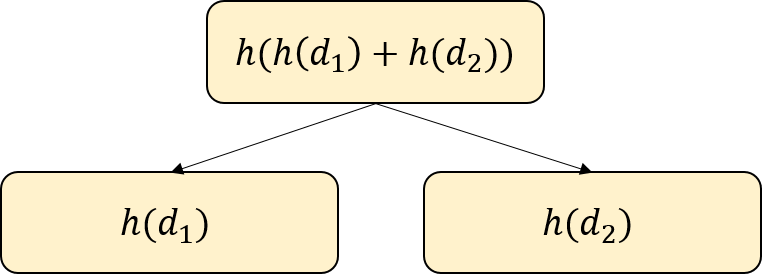
\includegraphics[scale=0.4]{dynamo/merkle-tree.png}
        \end{figure}
      \end{column}
    \end{columns}
    \begin{itemize}
      \item Consentono di identificare efficientemente differenze tra due alberi.
      \item Ogni nodo memorizza un Merkle tree per ogni intervallo che memorizza.
    \end{itemize}
  \end{block}
\end{frame}


\begin{frame}
  \frametitle{Membership e Rilevamento Fallimenti}
  \begin{block}{Gestire l'appartenenza al sistema (membership)}
  \begin{itemize}
  \item Non è presente una vista centralizzata dei membri appartenenti al sistema.
  \item Le informazioni sui membri sono scambiate mediante un protocollo \alert{gossip based}.
  \item Presenza di nodi \alert{seed} individuati ``staticamente'', notificati immediatamente dei cambiamenti nel sistema.
  \end{itemize}
  \end{block}
  \begin{block}{Rilevamento fallimenti}
  \begin{itemize}
  \item Il concetto di fallimento è locale.
    %per A il nodo B è fallito se non risponde, indipendentemente dalle risposte che può dare agli altri nodi.
  \item Dunque non c'è una visione unica e coerente dei nodi falliti, necessario un monitoring periodico.
  \end{itemize}
  \end{block}
  %$\longrightarrow$ Entrambe queste tecniche portano alta scalabilità.
\end{frame}


%% \begin{frame}
%%   \frametitle{Alcuni risultati}
%%   \begin{itemize}
%%   \item Dynamo è progettato per bilanciare consistency e availability.
%%   \item Come impattano differenti tipi di fallimenti sulla coerenza?
%%   \end{itemize}
  
%%   \begin{table}[ht]
%%   \begin{center} 
%%   \begin{tabular}{| r | r |}
%%   \hline  
%%   \textbf{\# Versioni} & \textbf{\% Client} \\   
%%   \hline
%%   \rowcolor{lightgray}
%%   1                              & 99.94 \\
%%   \hline
%%   2                              & 0.00057 \\
%%   \hline
%%   \rowcolor{lightgray}
%%   3                              & 0.00047 \\
%%   \hline
%%   4                              & 0.00009 \\ 
%%   \hline
%%   \end{tabular}
%%   \end{center}
%%   \end{table}

%%   \begin{itemize}
%%   \item La presenza di versioni divergenti è rara.
%%   \item L'esperimento ha evidenziato che la principale causa di incoerenze è un numero troppo eleveto di scritture concorrenti, spesso
%%     effettuate da bot e non da umani.
%%   \end{itemize}
%% \end{frame}


\begin{frame}
  \frametitle{Concludendo su Dynamo}
  \begin{block}{Vantaggi di Dynamo}
    \begin{itemize}
    \item Scalabilità.
    \item Riconciliazione versioni gestita dal client.
    \item Coerenza, availability, latency, regolabili appositamente per un'istanza.
    \end{itemize}
  \end{block}
  \begin{block}{Svantaggi}
  \begin{itemize}
  \item La riconciliazione a carico del client complica il codice delle applicazioni.
  \item Modificare dinamicamente i parametri $N, W, R$ per adattarsi alla situazione del sistema alleggerendo il traffico di richieste interne.
  \item Applicazioni client-side più complesse che prevedano l'arrivo di varie versioni e la loro riconciliazione.
  \end{itemize}
  \end{block}
\end{frame}

